\documentclass{beamer}

\usepackage[T2A]{fontenc}
\usepackage[utf8]{inputenc}
\usepackage[english,russian]{babel}
\usepackage{amssymb,amsfonts,amsmath,mathtext}
\usepackage{cite,enumerate,float,indentfirst}

\usepackage{graphicx}
\usepackage{booktabs}
\usepackage{tabularx}

\usepackage{qtree}    % regular trees (e.g. GB style)
\usepackage{gb4e}     % numbered lists for linguistic examples

\graphicspath{{images/}}

\usetheme{Rochester}
\usecolortheme{seagull}

\setbeamertemplate{footline}{\scriptsize{\hspace*{0.4cm}\insertframenumber}\vspace*{0.3cm}}
\beamertemplatenavigationsymbolsempty

\errorcontextlines 10000

\begin{document}

\title{\large{\sc Письменность и нормализация текста}}
\author{Константин Соколов}
\institute[]{СПбГПУ}
\date{Санкт-Петербург, 2015} 

\begin{frame}
    \thispagestyle{empty}
    \titlepage
\end{frame}


%%%%%%%%%%%%%%%%%%%%%
% 1. Повторение
%%%%%%%%%%%%%%%%%%%%%

\begin{frame}{}
\begin{center}
	\textbf{Повторение}
\end{center}
\end{frame}

\begin{frame}{Повторение}
\setcounter{framenumber}{1}
\begin{itemize}
    \item OpenCorpora
    \item слово, словоупотребление, словоформа, лексема, лемма
    \item предметный (объектный) язык и метаязык
\end{itemize}
\end{frame}


%%%%%%%%%%%%%%%%%%%%%%%%%%%%
% Письменность
%%%%%%%%%%%%%%%%%%%%%%%%%%%%

\begin{frame}{}
\begin{center}
	\textbf{Письменность}
\end{center}
\end{frame}

%     алфавитное и слоговое письмо, иероглифика; 
\begin{frame}{Алфавит}
\begin{figure}[H]
    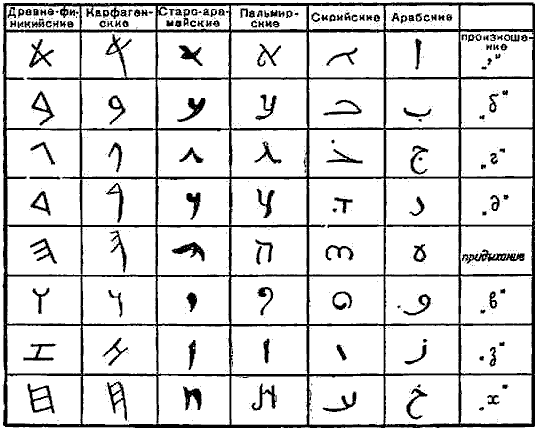
\includegraphics[scale=0.4]{alphabet.png} 
\end{figure}
\end{frame}

\begin{frame}{Силлабарий}
\begin{figure}[H]
    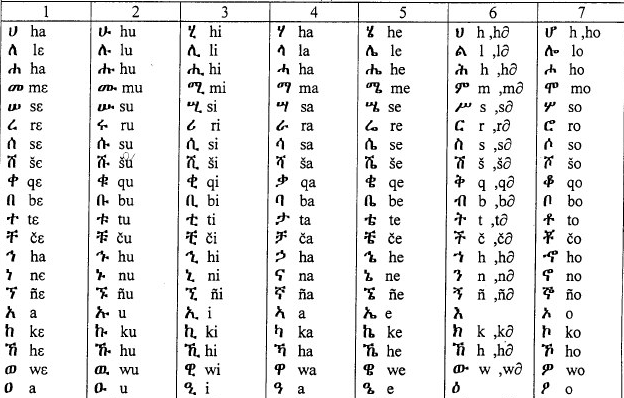
\includegraphics[scale=0.45]{amharic.png} 
\end{figure}
\end{frame}

\begin{frame}{Идеографика}
\begin{figure}[H]
    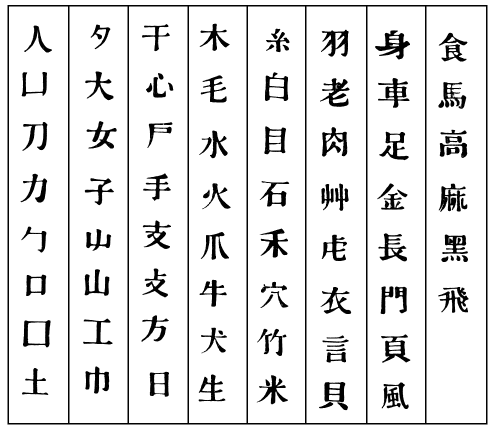
\includegraphics[scale=0.6]{ideographic.png} 
\end{figure}
\end{frame}

% ктив мале и ктив хасер; огласовки
\begin{frame}{Никуд}
\begin{figure}[H]
    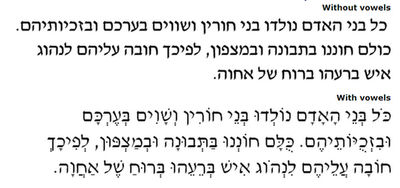
\includegraphics[scale=0.6]{hebrew.png} 
\end{figure}
\end{frame}

% направление письма
\begin{frame}{Двунаправленные тексты}
\begin{figure}[H]
    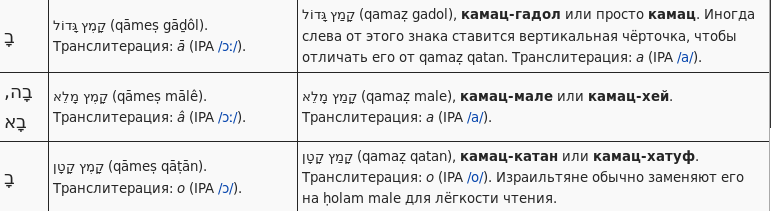
\includegraphics[scale=0.4]{bidirectional.png} 
\end{figure}
\end{frame}

% катакана, хирагана, кандзи, ромадзи
\begin{frame}{Кана}
\begin{figure}[H]
    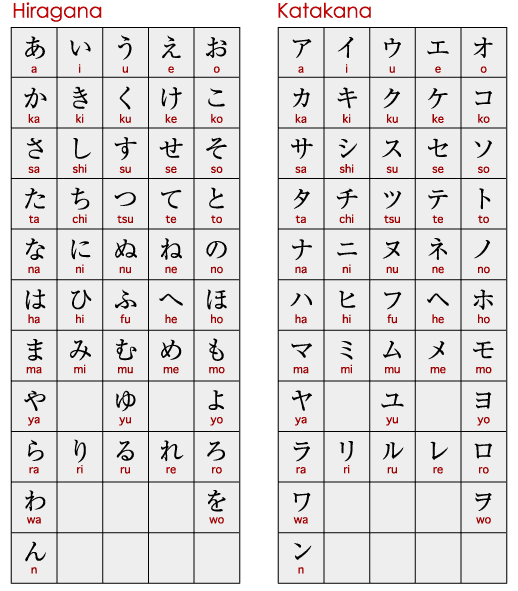
\includegraphics[scale=0.35]{kana.png} 
\end{figure}
\end{frame}

\begin{frame}{Кандзи}
\begin{figure}[H]
    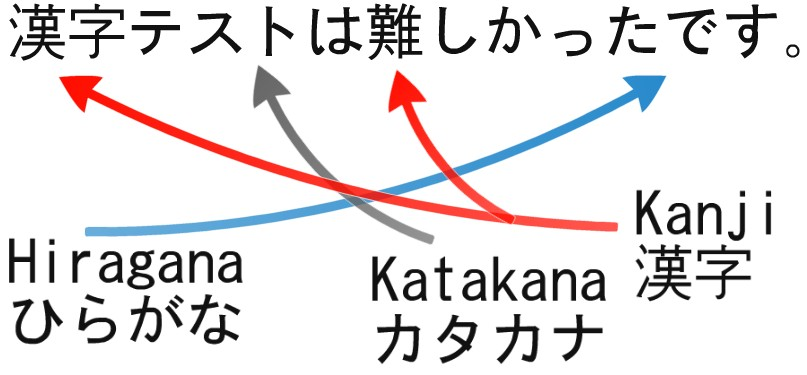
\includegraphics[scale=0.3]{kanji.jpg} 
\end{figure}
\end{frame}

%   диакритика 
\begin{frame}{Диакритика}
\begin{figure}[H]
    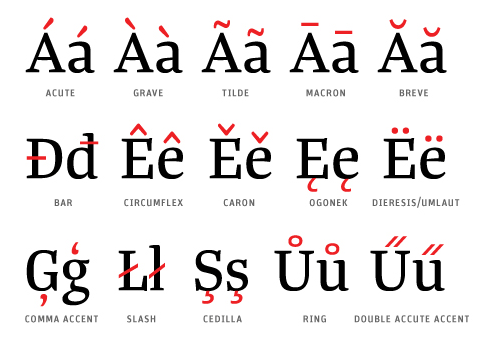
\includegraphics[scale=0.45]{diacritic.png} 
\end{figure}
\end{frame}

% лигатуры
\begin{frame}{Лигатуры (I)}
\begin{figure}[H]
    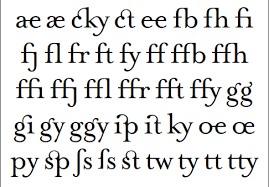
\includegraphics[scale=0.8]{ligatura.png} 
\end{figure}
\end{frame}

\begin{frame}{Лигатуры (II)}
\begin{figure}[H]
    
\includegraphics[scale=0.5]{devanagari.png} 
\end{figure}
\end{frame}

\begin{frame}{}
\begin{center}
	\textbf{Unicode}
\end{center}
\end{frame}

\begin{frame}{Графема}
\begin{itemize}
	\item аллограф (начертание) и графема
	\item глиф (glyph) и код (code point)
	    \begin{itemize}
	        \item примеры глифов: буквы (вкл. позиционные варианты), знаки препинания, акценты, огласовки, лигатуры и пр.
            \item пример code point: \texttt{U+0639} (hex)
	        \item ср. \textit{A} ($\langle a \rangle + \langle \equiv \rangle$) и \textit{а} ($\langle a \rangle$) у Глисона  и в Unicode
	    \end{itemize}
\end{itemize}
\end{frame}

% Unicode, представление диакритики в Unicode, нормализация Unicode); ICU (http://site.icu-project.org/)
\begin{frame}{Unicode (I)}
Необходимо различать три понятия:\\
\bigskip
\begin{itemize}
	\item character set -- неупорядоченный набор графических элементов
	\item coded character set -- набор кодов (абстрактных числовых идентификаторов графем)
	\item character encoding scheme -- кодировка (байтовое представление кодов)
\end{itemize}
\end{frame}

\begin{frame}{Unicode (II)}
combining characters -- глиф может образовываться с помощью базового символа и модификаторов\\
\medskip
\begin{figure}[H]
    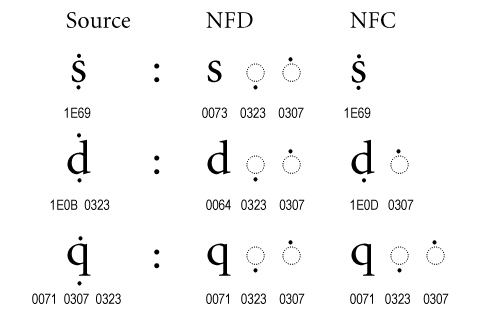
\includegraphics[scale=0.4]{combining.png} 
\end{figure}
\end{frame}

\begin{frame}{Unicode (III)}
\begin{figure}[H]
    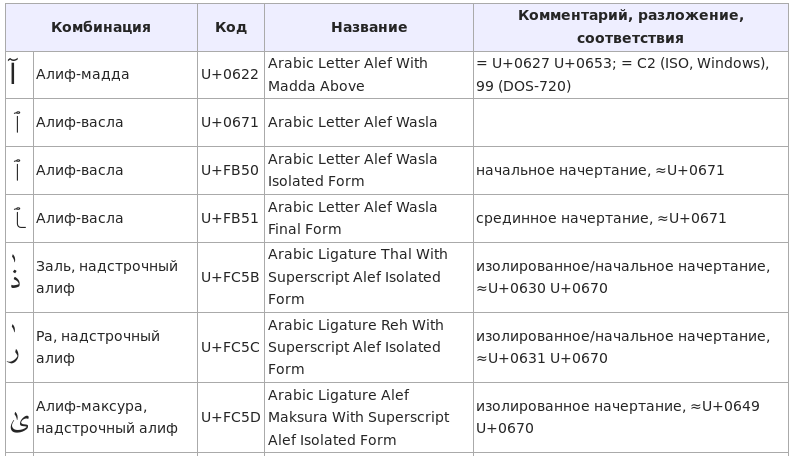
\includegraphics[scale=0.35]{combining-arabic.png} 
\end{figure}
\end{frame}

\begin{frame}{Unicode (IV)}
\begin{itemize}
	\item collation -- ``сортировка''
	    \begin{itemize}
	        \item в испанском диграф \textit{ch} трактуется как одна буква \textit{(c, ch, d)}
            \item \textit{\'{e}} может считаться эквивалентным \textit{e}
	        \item в немецком \textit{\"{a}} и \textit{ae} могут считаться эквивалентными
	        \item разный алфавитный порядок (лит.: \textit{i, y, k}; англ.: \textit{i, j, k})
	    \end{itemize}	
	\medskip
	\item кодировка
	    \begin{itemize}
	        \item UCS-2: 2 байта на code point 
            \item UTF-8: 1 байт для символов с code points < 127 (совпадает с ASCII), всего до 6 байтов на code point
            \item Byte Order Mark (\texttt{FF\,EF} vs. \texttt{EF\,FF})
	    \end{itemize}	
\end{itemize}
\end{frame}

\begin{frame}{Нормализация Unicode (I)}
\begin{itemize}
	\item Unicode Normalization Forms 
	    \begin{itemize}
	        \item \texttt{http://www.unicode.org/reports/tr15}
	    \end{itemize} 
	\medskip
	\item Два вида эквивалентности последовательностей символов
	    \begin{itemize}
	        \item canonical equivalence (напр., различные способы упорядочить модификаторы)
	        \item compatibility equivalence (напр., различные варианты, вкл. позиционные)
	    \end{itemize} 
\end{itemize}
\end{frame}

\begin{frame}{Нормализация Unicode (II)}
\begin{itemize}
	\item Нормальные формы определяются на основе композиции и декомпозиции code points
	    \begin{itemize}
	        \item NFD (Normalization Form D) -- каноническая декомпозиция
	        \item NFC -- каноническая декомпозиция, затем каноническая композиция
	        \item NFKD -- совместимая декомпозиция
	        \item NFKC -- совместимая декомпозиция, затем совместимая композиция
	    \end{itemize} 
\end{itemize}
\end{frame}

\begin{frame}{Нормализация Unicode (III)}
\begin{figure}[H]
    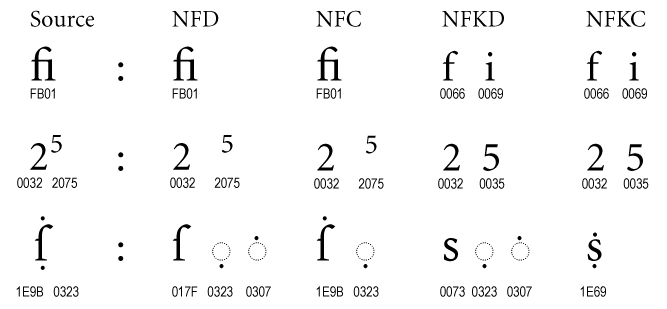
\includegraphics[scale=0.4]{normalized.png} 
\end{figure}
\end{frame}


%%%%%%%%%%%%%%%%%%%%%%%%%%%%
% Нормализация текста
%%%%%%%%%%%%%%%%%%%%%%%%%%%%

\begin{frame}{}
\begin{center}
	\textbf{Нормализация текста}
\end{center}
\end{frame}

\begin{frame}{Предобработка}
\begin{itemize}
	\item сегментация -- определение границ слов и предложений
	    \begin{itemize}
	        \item пунктуация, но ср.: \textit{В 2014 г. Сочи принимает Олимпиаду.}
	        \item фонотактика и консонантные кластеры
	        \item лингвостатистика и коллокации
	    \end{itemize}
	\item токенизация -- этап лексического анализа
	    \begin{itemize}
	        \item неоднозначность
	        \item \textit{французско-русский словарь} (4 токена)
	        \item ошибки токенизатора в OpenCorpora
	    \end{itemize}
\end{itemize}
\end{frame}

\begin{frame}{Стемминг и лемматизация}
\begin{itemize}
    \item стемминг -- получение неизменяемой части словоформы
        \begin{itemize}
            \item стеммер Портера и Snowball
            \item правила и эвристики
        \end{itemize}
	\item лемматизация -- получение леммы по словоформе
        \begin{itemize}
            \item неоднозначность
            \item словарная информация 
            \item необходимость предсказание слов, отсутствующих в словаре
            \item требования к эффективности
        \end{itemize}
\end{itemize}
\end{frame}


%%%%%%%%%%%%%%%%%%%%%%%%%%
% Дорожка
%%%%%%%%%%%%%%%%%%%%%%%%%%

\begin{frame}{}
\begin{center}
	\textbf{Shared Task / Дорожка}
\end{center}
\end{frame}

\begin{frame}{Стандартная процедура}
\begin{itemize}
    \item объявление условий и сроков
    \item публикация тестового корпуса
    \item публикация конкурсного корпуса
    \item подача результатов работы на конкурсном корпусе участниками
    \item объявление результатов организаторами
    \item подача статей, рецензирование
    \item очное представление систем (доклады)
\end{itemize}
\end{frame}

\begin{frame}{Учебная дорожка}
\begin{center}
Дорожка посвящена исследованию вопроса \\о влиянии стемминга на качество информационного поиска
\end{center}
\end{frame}

\begin{frame}{Условия}
\begin{itemize}
    \item командная разработка
    \item работа с русским языком
    \item \textbf{разрешается} использование любых алгоритмов стемминга, включая словарные (porter, snowball, 
      mystem, stemka, что найдете) и любых БД для хранения данных (при необходимости)
    \item \textbf{запрещается} использование любых движков полнотекстового поиска (Solr/Lucene, Sphinx и т.п.) 
      и средств полнотекстового поиска в БД
\end{itemize}
\end{frame}

\begin{frame}{Задание}
\begin{itemize}
	\item необходимо реализовать систему поиска документов в коллекции по инвертированному индексу
    \item система должна уметь:
        \begin{itemize}
            \item построить индекс для текстовой коллекции
            \item принимать текстовые запросы
            \item возвращать (отранжированный) список документов
        \end{itemize}
    \item описание языка запросов:
       \begin{itemize}
            \item словоформы разделяются пробелом (или несколькими) -- поиск всех слов
            \item текст в двойных кавычках -- поиск точного вхождения
            \item обработка пунктуации, спецсимволов и пр. -- по усмотрению участников
        \end{itemize}    
\end{itemize}
\end{frame}

\begin{frame}{Оценка результатов}
\begin{itemize}
	\item для оценки результатов будет предоставлен тестовый корпус и набор тестовых запросов
    \item результат работы системы должен быть предоставлен в CSV
    \item в качестве baseline-системы используется полнотекстовый поиск в PostgreSQL
    \item качество работы системы оценивается с помощью метрик полноты, точности и F-меры на основе экспертных оценок релевантности 
\end{itemize}
\end{frame}

\begin{frame}{Обзор данных}
50 текстов из OpenCorpora, 29890 с/у\\
\bigskip
\begin{itemize}
    \item художественная литература, писатели
    \item книги, издетельское дело, типографии, верстка
    \item галереи, искусство, авангард
    \item финансы, экономика, деньги
    \item компьютерные технологии
    \item без рубрики (шум)
\end{itemize}
\end{frame}

\begin{frame}[fragile]{Baseline -- I}
\begin{verbatim}
CREATE TABLE document
(
  id integer NOT NULL,
  text text,
  url text,
  CONSTRAINT document_pkey PRIMARY KEY (id)
);
\end{verbatim}
\end{frame}

\begin{frame}[fragile]{Baseline -- II}
\begin{footnotesize}
\begin{verbatim}
track1=# \dF
               List of text search configurations
   Schema   |    Name    |              Description
------------+------------+---------------------------------------
 pg_catalog | danish     | configuration for danish language
 pg_catalog | dutch      | configuration for dutch language
 pg_catalog | english    | configuration for english language
 pg_catalog | finnish    | configuration for finnish language
 pg_catalog | french     | configuration for french language
 pg_catalog | german     | configuration for german language
 pg_catalog | romanian   | configuration for romanian language
 pg_catalog | russian    | configuration for russian language
 pg_catalog | simple     | simple configuration
 pg_catalog | spanish    | configuration for spanish language
 ...
(16 rows)
\end{verbatim}
\end{footnotesize}
\end{frame}

\begin{frame}[fragile]{Baseline -- III}
\begin{footnotesize}
\begin{verbatim}
track1=# ALTER DATABASE track1 
track1=# SET default_text_search_config = 'pg_catalog.russian';
ALTER DATABASE

track1=# select to_tsvector('ворон к ворону летит 
track1=# ворон ворону кричит');
                     to_tsvector
-----------------------------------------------------
 'ворон':1,5 'ворону':3,6 'к':2 'кричит':7 'летит':4
(1 row)
\end{verbatim}
\end{footnotesize}
\end{frame}

\begin{frame}[fragile]{Baseline -- IV}
\begin{footnotesize}
\begin{verbatim}
track1=# CREATE TEXT SEARCH CONFIGURATION 
track1=# public.fts_config ( COPY=pg_catalog.russian );
CREATE TEXT SEARCH CONFIGURATION

track1=# CREATE TEXT SEARCH DICTIONARY russian_stem 
track1=# ( TEMPLATE=snowball, 
track1=# language='russian', stopwords='russian' );
CREATE TEXT SEARCH DICTIONARY
\end{verbatim}
\end{footnotesize}
\end{frame}

\begin{frame}[fragile]{Baseline -- V}
\begin{footnotesize}
\begin{verbatim}
track1=# SET default_text_search_config = 'public.fts_config';
SET

track1=# select to_tsvector('ворон к ворону летит 
track1=# ворон ворону кричит');
           to_tsvector
----------------------------------
 'ворон':1,3,5,6 'крич':7 'лет':4
(1 row)
\end{verbatim}
\end{footnotesize}
\end{frame}

\begin{frame}[fragile]{Baseline -- VI}
\begin{footnotesize}
\begin{verbatim}
track1=# select to_tsquery('книги | павича');
    to_tsquery
------------------
 'книг' | 'павич'
(1 row)

track1=# select to_tsquery('(книги | журналы) & павича');
           to_tsquery
---------------------------------
 ( 'книг' | 'журнал' ) & 'павич'
(1 row)

track1=# select plainto_tsquery('книги павича');
 plainto_tsquery
------------------
 'книг' & 'павич'
(1 row)
\end{verbatim}
\end{footnotesize}
\end{frame}

\begin{frame}[fragile]{Baseline -- VII}
\begin{footnotesize}
\begin{verbatim}
track1=# select count(*) from "document" 
track1=# WHERE "text" @@ 'книги и журналы';
 count 
-------
     1
(1 row)

track1=# select count(*) from "document" 
track1=# WHERE "text" @@ plainto_tsquery('книги и журналы');
 count 
-------
     1
(1 row)
\end{verbatim}
\end{footnotesize}
\end{frame}

\begin{frame}[fragile]{Baseline -- VIII}
\begin{footnotesize}
\begin{verbatim}
track1=# select count(*) from "document" 
track1=# WHERE "text" @@ to_tsquery('книги & журналы');
 count 
-------
     1
(1 row)

track1=# select count(*) from "document" 
track1=# WHERE "text" @@ to_tsquery('книги | журналы');
 count 
-------
    13
(1 row)
\end{verbatim}
\end{footnotesize}
\end{frame}

\begin{frame}[fragile]{Baseline -- IX}
\begin{footnotesize}
\begin{verbatim}
baseline> владел русским
[19]
baseline> Владел русским
[19]
baseline> владела русским
[19]
baseline> Владела русским
[19]
baseline> "владел русским"
[]
baseline> "Владел русским"
[19]
baseline> "Владела русским"
[]
baseline> "владела русским"
[]
\end{verbatim}
\end{footnotesize}
\end{frame}

\begin{frame}{Оценка -- I}
\begin{itemize}
    \item группы документов по отношению к запросу
        \begin{itemize}
            \item[A:] релевантные документы, попавшие в выдачу
            \item[B:] нерелевантные документы, попавшие в выдачу
            \item[C:] релевантные документы, не попавшие в выдачу
            \item[D:] нерелевантные документы, не попавшие в выдачу
        \end{itemize}
    \item мы хотим, чтобы в выдачу попадали все релевантные \\и только они (т.е., чтобы B и С были равны 0)
\end{itemize}
\end{frame}

\begin{frame}{Оценка -- II}
\begin{itemize}
    \item точность (precision) -- отношение найденных релевантных документов к общему количеству найденных документов
    \item полнота (recall) -- отношение найденных релевантных документов к общему количеству релевантных документов
\end{itemize}
\medskip
Например, всего 50 документов, из них 25 релевантны, \\при этом найдено 19, из них 8 релевантны. P = 8/19, R = 8/25
\end{frame}

\begin{frame}{Оценка -- III}
$F_1 = 2/(P^{-1} + R^{-1})$\\
\medskip
\begin{itemize}
    \item $0 \leqslant F_1 \leqslant 1$
    \item при $P = 0$ или $R = 0$ $F_1 = 0$
    \item если $P = R$, то $F_1 = P = R$
    \item $F_1 \geqslant min(P, R)$
    \item $F_1 \leqslant (R+P)/2$
\end{itemize}
\end{frame}

\begin{frame}[fragile]{Дорожка №1 (формат представления результатов)}
CSV, UTF-8, матрица запрос-документ, есть/нет в выдаче
\begin{footnotesize}
\begin{verbatim}
"query";"3";"7";"10";"14";"19";"24";"30";"54"
1;1;0;1;1;0;1;1;0
2;0;0;1;1;0;1;1;0
3;1;1;1;0;0;1;1;0
4;1;0;1;1;0;0;1;0
5;1;0;1;1;0;1;1;0
\end{verbatim}
\end{footnotesize}
\end{frame}

\begin{frame}[fragile]{Дорожка}
\begin{scriptsize}
\begin{verbatim}
baseline.csv

запрос                                   P       R       F1

астрономические обсерватории            	100.0	100.0	100.0
кинематография                          	100.0	33.0 	49.62
коллективизация                         	100.0	100.0	100.0
политические новости                    	0.0  	0.0  	NaN
экономический кризис                    	60.0 	42.0 	49.41
электронные издания                     	100.0	60.0 	75.0
\end{verbatim}
\end{scriptsize}
\end{frame}

\begin{frame}{}
    \thispagestyle{empty}
    \begin{center}
        {\large Спасибо!}
    \end{center}
\end{frame}


\end{document}
